\documentclass[preview]{standalone}

\usepackage{amsmath}
\usepackage{amssymb}
\usepackage{tikz}
\usepackage{wrapfig}
\usepackage{bettelini}
\usepackage{stellar}
\usepackage{definitions}

% =======
\usetikzlibrary{ % tikz packages
    automata,positioning,
    arrows.meta,bending
}
\tikzset{every state/.style={
    inner sep=2pt,
    minimum size=4pt
}}
\tikzset{>=stealth}  %latex, to, stealth
% Empty string symbol.
\newcommand{\emptyString}{\lambda}
% =======

\begin{document}

\id{theoryofcomputation-dfa}
\genpage


\section{Deterministic Finite Automaton}

\begin{snippetdefinition}{dfa-definition}{Deterministic Finite Automaton}
    A deterministic finite automaton (DFA) is a state-machine which processes a string
    symbol by symbol from left to right. The automaton is in one of his \textit{states}
    after processing a symbol. The machine might terminate in an
    \textit{accept state} or not.

    A DFA \(M=(Q, \Sigma, \delta, q, F)\)
    \begin{itemize}
        \item \(Q\) is a finite set of \textit{states}
        \item \(\Sigma\) is an alphabet
        \item \(\delta \colon Q \cartesianprod \Sigma \fromto Q\) is the \textit{transition function}
        \item \(q\) is an element of \(Q\) called the \textit{start state}
        \item \(F\) is a subset of \(Q\) which contains the \textit{accept states}
    \end{itemize}
    The transition function is the logical components, it determines
    in which state the machine will be after processing a symbol at any state.

    If a DFA is in a state \(r\) and it reads the symbol \(a\),
    then it will uniquely switch to the state \(\delta(r, a)\)
\end{snippetdefinition}

\begin{snippetexample}{dfa-example}{DFA Example}
    The following automaton processes a binary string.
    The start state is \(q_1\) and the only accept state is \(q_3\).
    The program moves to the next state only if the symbol is \(1\),
    so it will reach \(q_3\) only if the input string contains at least two \(1\)s.
    \begin{center}
        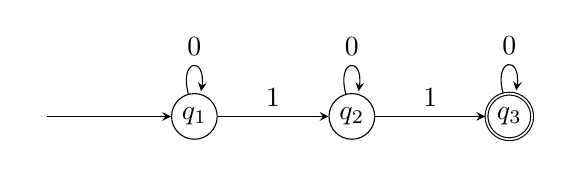
\begin{tikzpicture}[node distance=2cm,on grid,auto]
            \node[state] (q1) {\(q_1\)};
            \node (inv) [left=of q1] {};

            \node[state] (q2) [right=of q1] {\(q_2\)};
            \node[state, accepting] (q3) [right=of q2] {\(q_3\)};

            \path[->]
                (inv)
                    edge node {} (q1)
                (q1)
                    edge node {\(1\)} (q2)
                    edge[loop above] node {\(0\)} ()
                (q2)
                    edge node {\(1\)} (q3)
                    edge[loop above] node {\(0\)} ()
                (q3)
                    edge[loop above] node {\(0\)} ();
        \end{tikzpicture}
    \end{center}
\end{snippetexample}

\begin{snippetdefinition}{languages-of-automaton-definition}{Languages of automaton}
    The language of \(M\), denoted \(L(M)\) is the set of all accepted strings
    by \(M\).
    \[
        L(M) \triangleq \{w \in \Sigma^* \suchthat M\text{ accepts }w\}
    \]
\end{snippetdefinition}

\end{document}